\usetikzlibrary{matrix}
\usetikzlibrary{shapes,snakes}
	\tikzstyle{rec} = [rectangle, rounded corners, minimum width=1cm, minimum height=1cm,text centered, draw=black]
	\tikzstyle{circ} = [circle,minimum size =1.5cm,text centered, draw=black]
	\tikzstyle{arrow} = [thick,->,>=stealth]
		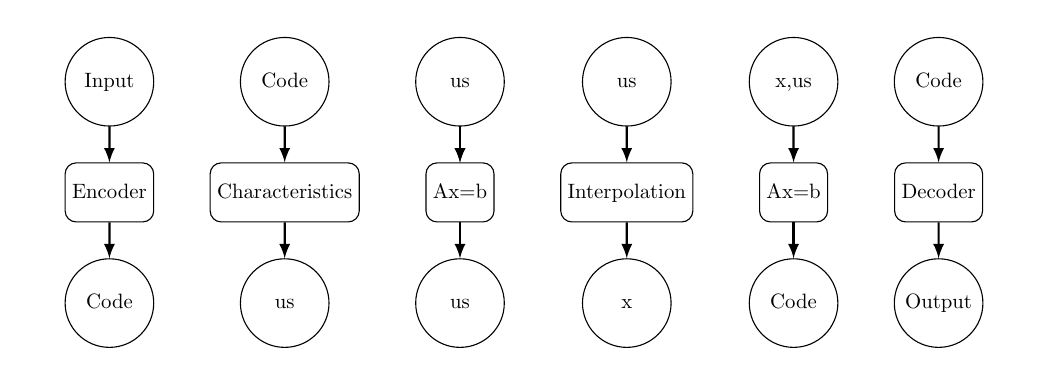
\begin{tikzpicture}[>=latex,text height=1.5ex,text depth=0.25ex,scale=.5,every node/.style={scale=0.75}]
		\matrix[matrix of nodes,column sep= 1em,row sep= 3ex]{
			&
			\node[circ] (1) {Input};&
			&
			\node[circ] (4) {Code};&
			&
			\node[circ] (7) {us};&
			&
			\node[circ] (10) {us};&
			&
			\node[circ] (13) {x,us};&
			&
			\node[circ] (16) {Code};&
			\\
			&
			\node[rec] (2) {Encoder};&
			&
			\node[rec] (5) {Characteristics};&
			&
			\node[rec] (8) {Ax=b};&
			&
			\node[rec] (11) {Interpolation};&
			&
			\node[rec] (14) {Ax=b};&
			&
			\node[rec] (17) {Decoder};&
			\\
			&
			\node[circ] (3) {Code};&
			&
			\node[circ] (6) {us};&
			&
			\node[circ] (9) {us};&
			&
			\node[circ] (12) {x};&
			&
			\node[circ] (15) {Code};&
			&
			\node[circ] (18) {Output};&
			\\
		};
	\path[->]
		(1) edge[thick] (2)
		(2) edge[thick] (3)
		(4) edge[thick] (5)
		(5) edge[thick] (6)
		(7) edge[thick] (8)
		(7) edge[thick] (8)
		(8) edge[thick] (9)
		(10) edge[thick] (11)
		(11) edge[thick] (12)
		(13) edge[thick] (14)
		(14) edge[thick] (15)
		(16) edge[thick] (17)
		(17) edge[thick] (18);
\end{tikzpicture}